\chapter{Example Algorithm} \label{Algorithm}

An example algorithm for compressed branch trace is given in figure~\ref{fig:algo}. 
In the diagram, the following terms are used:

\begin{itemize}
  \item \textit{Qualified?}  An instruction that meets the filtering criteria is qualified, and will be traced;
  \item \textit{Branch?} Is the instruction a branch or not (\textbf{itype} values 4 or 5, or a non-zero \textbf{ntkn});
  \item \textit{branch map.}  A vector where each bit represents the outcome of a branch.  A 0 indicates the
    branch was taken, a 1 indicates that it was not;
  \item \textit{inst.}  Abbreviation for 'instruction';
  \item \textit{resync count.} A counter used to keep track of when it is necessary to send 
    a synchronization packet (see Section~\ref{synchronization}, final bullet). The exact mechanism for 
    incrementing this counter are not specified, but options might be to count the number of \textit{te\_inst} packets emitted, 
    or the number of clock cycles elapsed since the last synchronization message was sent;
  \item \textit{max\_resync.}  The resync counter value that schedules a synchronization packet;
  \item \textit{updiscon.}  Uninferable PC disconinuity.  This identifies an instruction that
    causes the program counter to be changed by an amount that cannot be predicted from the
    source code alone (\textbf{itype} values 6, 7, 8, 10, 12 or 14);
   \item \textit{te\_inst.} The name of the packet type emitted by the encoder (see Chapter~\ref{packets});
   \item \textit{e\_ccd.} An exception has been signalled, or context has changed and
     should be treated as an uninferable PC discontinuity (see Table~\ref{tab:context-type});
   \item \textit{ppch.} Privilege has changed, or context has changed and needs to be 
     reported precisely (see Table~\ref{tab:context-type});
   \item \textit{ppch\_br.} As above, but branch map not empty;
   \item \textit{resync\_br.} The resync counter has reached the maximum value and there are
     entries in the branch map that have not yet been output.  These must be output before
     the subsequent synchronization packet, which does not report branch map history;
   \item \textit{er\_ccdn.}  Instruction retirement and exception signalled on the same cycle, 
     or context has changed and should be treated as an uninferable PC discontinuity, or
     context notify (see Table~\ref{tab:context-type});
   \item \textit{exc\_only.}  Exception signaled without simultaneous retirement;
   \item \textit{cci.}  context change that can be reported imprecisely (see Table~\ref{tab:context-type}).
\end{itemize}

\begin{figure}[l]
\begin{center}
  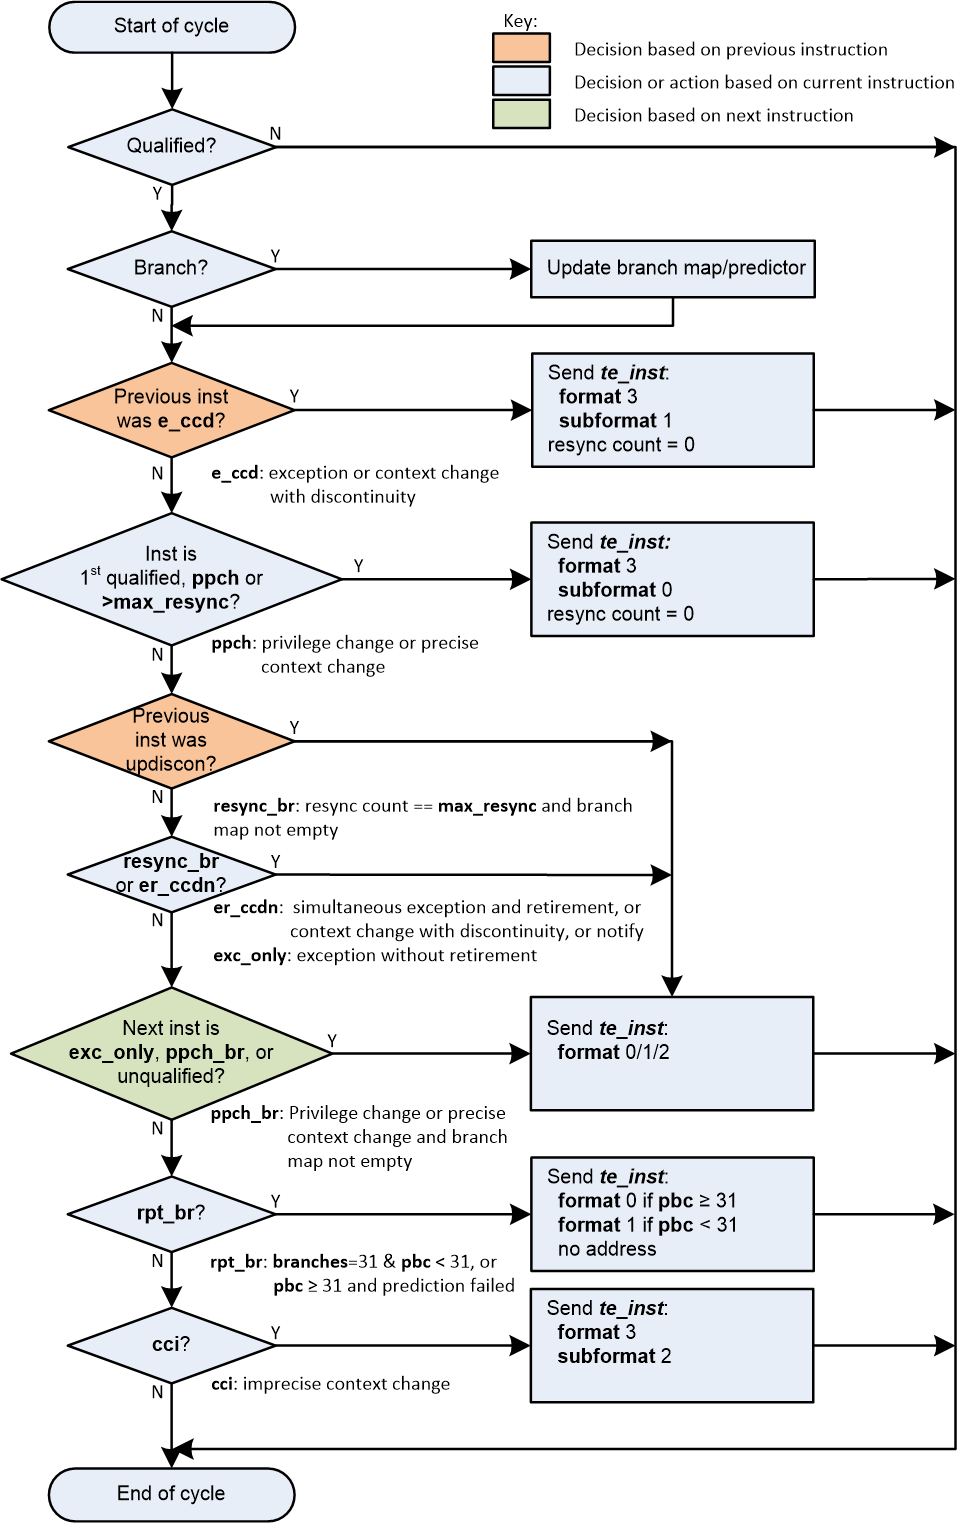
\includegraphics[height=23cm, width=15cm]{algo.png}
  \caption{Delta Mode 1 instruction trace algorithm}
  \label{fig:algo}
\end{center}
\end{figure}

Figure~\ref{fig:algo} shows instruction by instruction behavior, as would be
seen in a single-retirement system only.  Whilst the ingress port allows the RISC-V core to
provide information on multiple retiring instructions simultaneously, the resultant packet
sequence generated by the encoder must be the same as if retiring one instruction at a time.

A 3-stage pipeline is assumed, such that the encoder has 
visibility of the current, previous and next instructions.  All packets are generated using 
information relating to the current instruction.  The orange diamonds indicate decisions 
based on the previous (or last) instruction, the green diamond indicates a decision based on the
next instruction, and all other diamonds are based on the current instruction.

Additionally, the encoder can generate two further packet types, not shown on the diagram for 
clarity (see Chapter~\ref{packets}):

\begin{itemize}
  \item a \textit{te\_support} packet is sent when the encoder is enabled or disabled, or its
    configuration is changed, and also after the last qualified instruction has been traced.
    This informs the decoder of the operating mode of the encoder, and also that tracing has
    stopped;
  \item a \textit{packet\_lost} packet is sent if trace packets are lost (for example if the 
    buffer into which packets are being written fills up.  In this situation, the 1st packet 
    loaded into the buffer when space next becomes available should be a \textit{packet\_lost} 
    packet.  Following this, tracing will resume with a sync packet.
\end{itemize}

Note: if the \textbf{halted} or \textbf{reset} sideband signals are asserted (see Table~\ref{tab:ingress-side-band})
the encoder will behave as if it has received an unqualified instruction (output \textit{te\_inst}
reporting the address of the last instruction, followed by \textit{te\_support});

\section{Full vs Differential Addresses} \label{addresses}
In all cases but one, the packet format is determined only by a 'yes' outcome from the 
associated decision.  The choice between format 0, 1 or 2 for the case in the middle of the 
diagram needs further explanation.  

Addresses can be output in one of two ways: \textit{full} or \textit{differential}.

\begin{itemize}
  \item The \textit{full} address is the actual address of the current instruction;
  \item The \textit{differential} address is the difference between the actual address of 
    the current instruction and the actual address of the instruction reported in the 
    previous packet that contained an address.
\end{itemize}

Packet formats 0 and 1 include the full or differential address respectively, along with a 
branch map.  If the branch map is not empty, The choice of which format to use is determined as follows:

\begin{enumerate}
  \item Calculate the differential address (current address minus previously reported address);
  \item Count the number of identical most-significant bits for both the full and 
    differential addresses;
  \item Choose the address which has the highest number of identical bits.
\end{enumerate}

For example, suppose the current address is 0xffff1234, and the address of the instruction most
recently output in a packet is 0xffff1200.  The differential address is 0x00000034.  This has 
26 identical MSBs.  The full address has ony 16 identical MSBs, so the differential address is
chosen.

If the branch map is empty and does not need to be reported, packet format 2 is used.  This
always contains a differential address.  The rationale here is that if there are no branches to 
report then the instruction address is unlikely to differ by much from the previously reported
address, and so the differential form is much more likely to be optimal.  Offering a choice
between full and differential would require an extra bit in the packet, which would reduce the
efficiency.  

The packet formats are organized so that the address is always the final field.  Minimizing the 
number of bits required to represent the address reduces the total packet size and significantly
improves efficiency.  See Chapter~\ref{packets}.
